% ---------------------------------------------------------------------------
% arXiv abstract (plain text for the submission form; <= 1,900 characters):
%
% Adaptive systems change their own organization, and organization determines
% which recovery paths remain reachable. We compare four nested control classes
% along the same baseline (the incumbent policy, any policy within current
% capabilities, attainable capability changes, and an idealized physical
% planner) using finite-horizon viability kernels. This yields a five-level
% severity taxonomy and a point of no return for each class; the interval
% between the last two is organizational lock-in, where physical recovery
% remains possible but no admissible reorganization reaches it. In an exactly
% solved settlement model, organization alone sets severity, and a rule that
% maximizes food stored over the next two ticks and favors foraging on ties
% enters lock-in while holding more food than a generalist that can still
% retrain. Across 6,000 settings this selection is tie-breaking without
% friction and becomes strict once training costs one food per trainee-tick; a
% viability shield survives every setting. Necessity of acceleration is a
% kernel condition, and along the incumbent path delay never lowers the
% required rate under an unchanged, nested ceiling. In a stylized climate
% model, capacity building closes the headline 2C window in 2040 versus 2045
% with unlimited capacity, and acceleration without a stopping rule closes it
% two to six years earlier. A machine-checked reduction from bounded STRIPS
% planning makes deciding escape PSPACE-hard with a binary horizon; checking a
% restoration seed set is linear-time but choosing a smallest one is a directed
% feedback vertex set problem, and a robust optimizer over a finite threat set
% never buys a costly cycle-breaking seed. General propositions are proved in
% Lean 4; settlement facts are certified by computation; climate results are
% numerical, cross-checked, and conditional on a stylized model.
% ---------------------------------------------------------------------------
\documentclass[11pt]{article}

\usepackage[utf8]{inputenc}
\usepackage[T1]{fontenc}
\usepackage[margin=1in]{geometry}
\usepackage{amsmath}
\usepackage{amssymb}
\usepackage{amsthm}
\usepackage{mathtools}
\usepackage{graphicx}
\usepackage{booktabs}
\usepackage{array}
\usepackage{xcolor}
\usepackage[shortlabels]{enumitem}
\usepackage{microtype}
\usepackage[authoryear,round]{natbib}
\usepackage[colorlinks=true,linkcolor=blue!50!black,citecolor=blue!50!black,urlcolor=blue!50!black]{hyperref}

\setlist{itemsep=2pt,topsep=4pt}

\theoremstyle{plain}
\newtheorem{theorem}{Theorem}
\newtheorem{proposition}[theorem]{Proposition}
\newtheorem{corollary}[theorem]{Corollary}
\newtheorem{lemma}[theorem]{Lemma}
\theoremstyle{definition}
\newtheorem{definition}{Definition}

\newcommand{\K}{\mathcal{K}}
\newcommand{\V}{\mathcal{V}}
\newcommand{\W}{\mathcal{W}}
\newcommand{\U}{\mathcal{U}}
\newcommand{\M}{\mathcal{M}}
\newcommand{\A}{\mathcal{A}}
\newcommand{\CapStr}{\mathcal{C}}
\newcommand{\fixed}{\mathrm{fixed}}
\newcommand{\policy}{\mathrm{policy}}
\newcommand{\adapt}{\mathrm{adapt}}
\newcommand{\phys}{\mathrm{phys}}
\newcommand{\fail}{\mathrm{fail}}
% Lean identifiers in typewriter type; allow line breaks after underscores.
\newcommand{\lean}[1]{{\ttfamily\renewcommand{\_}{\textunderscore\allowbreak}#1}}
\newcolumntype{L}[1]{>{\raggedright\arraybackslash}p{#1}}

\hypersetup{
  pdftitle={The Paradox of Adaptive Organization},
  pdfauthor={Patrick Barletta}
}

\title{The Paradox of Adaptive Organization:\\
Organizational Lock-in, the Necessity of Acceleration,\\
and the Adaptive Escape Problem}
\author{Patrick Barletta}
\date{November 2026}

\begin{document}
\maketitle

\begin{abstract}
Adaptive systems change their own organization, and organization determines which recovery paths remain reachable. We compare four nested control classes along one baseline (the incumbent policy, any policy within current capabilities, attainable capability changes, and an idealized physical planner) using finite-horizon viability kernels. This yields a five-level severity taxonomy and a point of no return per class; the interval between the last two is \emph{organizational lock-in}, where physical recovery remains possible but no admissible reorganization reaches it. In an exact settlement model, organization alone sets severity, and a rule maximizing food stored over two ticks that favors foraging on ties enters lock-in while holding more food than a generalist that can still retrain. Across 6,000 settings this selection is tie-breaking without friction and strict once training costs food; a viability shield survives every setting. Necessity of acceleration is a kernel condition, and along the incumbent path delay never lowers the required rate under an unchanged, nested ceiling. In a stylized climate model, capacity building closes the headline 2$^\circ$C window in 2040 versus 2045 with unlimited capacity, and acceleration without a stopping rule closes it two to six years earlier. A machine-checked reduction from bounded planning makes deciding escape PSPACE-hard with a binary horizon; choosing a smallest restoration seed set is a directed feedback vertex set problem, and robust optimization over a finite threat set never buys a costly cycle-breaking seed. General propositions are proved in Lean~4; settlement facts are computer-certified; climate results are numerical and model-conditional.
\end{abstract}

\section{Introduction}
\label{sec:intro}

How long can a target remain physically achievable after an organization has lost the ability to reach it? Organizations build, specialize and discard capabilities, and each adaptation changes which actions, policies and further reorganizations are feasible. That efficiency need not buy resilience is a familiar theme \citep{LeonardBarton1992,March1991,RepenningSterman2002,CarlsonDoyle2002}. We make three narrower claims, each checkable.

\textbf{I. The paradox of adaptive organization.} Systems in the same physical state, environment and deadline can differ in severity purely because of their organization, and a short-horizon optimizer can select the locked-in side. In an exact settlement model, a rule that maximizes food stored over the next two ticks and favors foraging on ties enters lock-in; the same objective with ties favoring training preserves recovery. Under monotone dynamics, if a poorer state can reorganize and a richer one is locked in, their modeled organizations or commitments must differ.

\textbf{II. The necessity of acceleration.} When constraints change faster than adaptive processes respond, staying viable can require building capability faster. We state necessity as a kernel condition and prove that, along the incumbent trajectory, waiting under an unchanged rate ceiling can only raise the required rate. In a stylized climate model the binding constraint shifts, and acceleration without a stopping rule consumes its own margin.

\textbf{III. The adaptive escape problem.} Deciding whether some admissible sequence of reorganizations keeps a system viable inherits the worst-case hardness of planning. Exact or bounded computation remains possible under structure, and lock-in can be claimed only with a physical witness and an exclusion of the adaptive class.

\paragraph{What is machine-checked.} We distinguish three levels of assurance. (a)~\emph{General theorems} (nesting, monotone loss, resource monotonicity, the delay theorem, the planning--escape equivalence, the timed bootstrap, seed undervaluation) are proved in Lean~4 for abstract systems, without \lean{sorry} or \lean{native\_decide}. (b)~\emph{Model facts} for the one settlement model are certified by exhaustive computation in Lean using \lean{native\_decide}, which trusts the Lean compiler; theory and certified model are not formally linked. (c)~\emph{Numerical results} (climate sweeps, Experiment~E, friction sweep) come from Lean executables and are reproduced field by field by an independent Python implementation; the climate dominance arguments are proved on paper and checked numerically. Appendix~\ref{app:lean} lists theorem names and Appendix~\ref{app:repro} describes reproduction. The verified artifact is \url{https://github.com/Patrick-Barletta/Paradox_of_Adaptive_Organization} (release tag v1.0).

\paragraph{Evidentiary hygiene.} The settlement model establishes existence, not prevalence. Real-world episodes, such as the scheduling failure in a simulated settlement game that motivated this work, are illustrations, never certified classifications. Climate results are conditional on a stylized model and are not forecasts.

\section{Framework}
\label{sec:framework}

\subsection{State, moves and control classes}

The state is $s_t=(x_t,O_t,\pi_t,q_t)$: physical state $x$, organization $O$, operational policy $\pi$, and commitments $q$ (obligations and reorganizations in progress). The organization determines a \emph{capability structure} $\CapStr(O)=(\A(\cdot,O,\cdot),\Pi(O),\M(O,\cdot))$ of available actions, policies and moves. Time is discrete with fixed terminal time $T$, and the environment path $w_{0:T}$ is known in the deterministic version. Each tick the system revises its policy, chooses a move $m_t\in\M(O_t,q_t)$ (including the null move $\varnothing$), and executes a realizable action; $x$, $O$ and $q$ evolve as functions of $(x_t,O_t,q_t,a_t,m_t,w_t)$. A non-null move has latency $\tau(m)\ge1$, a resource draw, and a transitional restriction ($\A$ may shrink while it is pending: trainees cannot forage). Organization also drifts through attrition and skill loss.

\begin{definition}[Policy versus organizational change]
A move is \emph{capability-changing} if completing it alters $\CapStr(O)$, and an \emph{implementation} move if it only puts an already-admissible policy into effect. A change is \emph{organizational} if and only if it uses a capability-changing move; every other change, however slow or costly, is a \emph{policy} change.
\end{definition}

Four nested classes restrict continuations from an incumbent policy $\pi_0$: $\U_\fixed$ runs the incumbent unchanged (with a fallback map $\phi_O$ replacing unexecutable components by null actions); $\U_\policy$ allows free policy revision within $\Pi(O_t)$ with only null or implementation moves; $\U_\adapt$ also allows capability-changing moves; and $\U_\phys$ is an idealized planner acting directly on physical dynamics $f_\phys$, bypassing organization. Native reorganization routines are modeled as a baseline meta-policy $\mu_0$ retained by the fixed and policy classes.

The assumptions are: \textbf{A0}, viability and terminal sets depend only on $x$ ($\V=\V_x\times\mathcal O\times\Pi\times\mathcal Q$, $\W=\W_x\times\cdots\subseteq\V$), so institutional constraints enter only through admissible sets; \textbf{A1}, a costless null move and null action always exist; \textbf{A2}, every policy is total, with fallback-completed policies admissible in every reachable organization; \textbf{A3}, every admissible organizational step is reproduced by some physical action yielding the same next $x$. A3 may be replaced by a dominance version \textbf{A3$'$} under a preorder $\succeq$ that orders viability-relevant components favorably, with simulation and upward-closure conditions.

\subsection{Kernels, severity and points of no return}

\begin{definition}[Class kernels and severity]
For $k\in\{\fixed,\policy,\adapt,\phys\}$, $\K_k(t)$ is the set of states from which some class-$k$ continuation stays in $\V$ through $T$ and ends in $\W$. The \emph{severity} $\sigma(s,t)$ is 0 if $s\in\K_\fixed(t)$ (viable as-is); 1 if $s\in\K_\policy\setminus\K_\fixed$ (operational mismatch); 2 if $s\in\K_\adapt\setminus\K_\policy$ (recoverable organizational mismatch); 3 if $s\in\K_\phys\setminus\K_\adapt$ (structural organizational lock-in); and 4 if $s\notin\K_\phys$ (physical nonviability).
\end{definition}

With $\W=\V$ these are finite-horizon viability kernels \citep{Aubin1991}, computed in the deterministic case by backward recursion in the target-tube manner of \citet{BertsekasRhodes1971}.

\begin{proposition}[Nesting]\label{prop:nesting}
Under A0--A3 (or A0--A2 with A3$'$), $\K_\fixed(t)\subseteq\K_\policy(t)\subseteq\K_\adapt(t)\subseteq\K_\phys(t)$ for every $t$; hence the five severities partition the state space.
\end{proposition}
\begin{proof}[Proof sketch]
A fixed continuation is a policy continuation choosing $\phi_{O_t}\circ\pi_0$ (A2); a policy continuation is an adapt continuation; an adapt continuation is replaced step by step by the physical actions of A3, producing the same $x$-path, and viability depends only on $x$ (A0). Under A3$'$ induction builds a dominating path.
\end{proof}

The physical class relaxes organizational constraints, not the environment's response: if observers react to an announced move, $f_\phys$ must carry the same reaction, or $\K_\phys\setminus\K_\adapt$ mixes lock-in with a friendlier environment.

Let $s^{\mathrm b}_t$ be the baseline (incumbent) trajectory and $t_\fail$ the index of its first state outside $\V$. For $k\in\{\policy,\adapt,\phys\}$ the \emph{point of no return} is $t^*_k=\min\{t: s^{\mathrm b}_t\notin\K_k(t)\}-1$. This applies, class by class, the last-start idea known for vehicles as the time to react \citep{SoentgesEtAl2018}. By nesting, $t^*_\policy\le t^*_\adapt\le t^*_\phys<t_\fail$.

\begin{proposition}[Monotone loss, known environment path]\label{prop:monotone}
If $s^{\mathrm b}_t\in\V$ and $s^{\mathrm b}_{t+1}\in\K_k(t+1)$, then $s^{\mathrm b}_t\in\K_k(t)$. Hence before $t_\fail$ kernel membership along the baseline is exactly the prefix $[0,t^*_k]$.
\end{proposition}
\begin{proof}[Proof sketch]
The baseline step is admissible in every class (A1--A3); prepend it. The fixed terminal time is essential.
\end{proof}

If the baseline fails, the time before $t_\fail$ splits into a policy-recoverable segment $[0,t^*_\policy]$, the \emph{reorganization window} $(t^*_\policy,t^*_\adapt]$, the \emph{lock-in interval} $(t^*_\adapt,t^*_\phys]$ of length $\Delta_{\mathrm{lock}}=t^*_\phys-t^*_\adapt$, and a final segment with no recovery. ``Least permissive'' orders classes, not costs: a policy-class recovery can use more resources than an available reorganization. The \emph{organizational margin} $\mu(s,t)=t^*_\adapt(s,t)-t$ counts the ticks the incumbent can keep running before reorganization can no longer save it.

Under uncertainty, robust kernels still nest and partition, but Proposition~\ref{prop:monotone} fails as stated: if tomorrow brings either a harmless or a fatal disturbance, no strategy guarantees survival today, yet the realized successor can lie in the robust kernel. The robust analogue strengthens the premise.

\begin{proposition}[Robust monotone loss]\label{prop:robust}
If $s^{\mathrm b}_t\in\V$ and every possible baseline successor lies in the robust kernel $\K^{\mathrm{rob}}_k(t+1)$, then $s^{\mathrm b}_t\in\K^{\mathrm{rob}}_k(t)$, provided successors are distinguishable from the next observation.
\end{proposition}

Under uncertainty, $t^*_k$ therefore marks the last moment class-$k$ recovery is \emph{guaranteed}; a realized path can re-enter by luck. All classes must also share the same observation, or organizational lock-in mixes with informational loss.

\paragraph{Evidence standard.} Membership is constructive (one witness); exclusion is universal. Operational mismatch is the only failure class that can be established entirely by construction, and physical nonviability often has cheap certificates such as conservation or budget bounds. Lock-in is hardest, since it quantifies over sequences of reorganization moves. We therefore report a severity interval $[\sigma_{\min},\sigma_{\max}]$: a witness caps $\sigma_{\max}$; a certificate (exhaustive search over the whole class, an outer relaxation, or a solvability-preserving reduction) raises $\sigma_{\min}$; ``no witness under budget $B$'' is never an exclusion. Lock-in is claimed only when the interval is exactly $\{3\}$.

\section{The paradox of adaptive organization}
\label{sec:paradox}

\subsection{An exactly solved settlement}

Table~\ref{tab:settlement} specifies a deterministic settlement whose four kernels are computed exactly by backward recursion over all 17,136 time-indexed states. Every membership claim has a witness re-verified by forward simulation; every exclusion is exhaustive. The model satisfies A3$'$, and nesting is confirmed numerically (0 violations).

\begin{table}[t]
\centering\small
\caption{The settlement model.}
\label{tab:settlement}
\begin{tabular}{@{}lL{4.4in}@{}}
\toprule
Component & Specification \\
\midrule
Workers & $N=3$; each eats 1 food per tick \\
$x=(F,P)$ & food stock $F\in\{0,\dots,20\}$ (cap 20, surplus discarded); harvest $P$ arriving next tick \\
$O$, $q$ & farming capability, whether foragers are specialized; worker-ticks of training completed \\
Environment & wild yield per forager 2 for $t<6$, 1 for $6\le t<8$, 0 after; $T=16$ \\
Forage, farm & wild yield per forager, $+1$ if specialized and yield $>0$; farm: 2 per farmer, next tick \\
Moves & train: farming after 2 worker-ticks (generalists) or 8 (specialists); specialize: irreversible \\
$\V$ & no starvation: $F+\text{forage}+P-N\ge0$ every tick \\
Classes & fixed: all forage; policy: any allocation to forage, farm (if capable), idle; adapt: plus training and specialization; phys: farming without training, best foraging technique \\
\bottomrule
\end{tabular}
\end{table}

\paragraph{Organization alone sets severity.} Table~\ref{tab:states} shows five states at $t=11$. The $\sigma=1,2,3$ states share time, environment and physical state and differ \emph{only in organization}. The locked-in specialists' physical recovery is exactly the plan the farm-capable settlement executes at $\sigma=1$; they cannot reach it because eight worker-ticks of retraining with no food coming in exhaust the stock before the first harvest. Generalists need two.

\begin{table}[t]
\centering\small
\caption{Five demonstration states at $t=11$; all classifications exact.}
\label{tab:states}
\begin{tabular}{@{}clll@{}}
\toprule
$\sigma$ & State & Least permissive witness & Exhaustively excluded \\
\midrule
0 & $F=16$, no farm, generalists & incumbent forages to $T$ & none \\
1 & $F=9$, farm, generalists & farm 2 at $t=13$, 1 at $t=14$ & $\K_\fixed$ \\
2 & $F=9$, no farm, generalists & train 2 at $t=12$, then farm & $\K_\fixed,\K_\policy$ \\
3 & $F=9$, no farm, specialists & phys.: farm 2 at $t=13$, 1 at $t=14$ & $\K_\fixed,\K_\policy,\K_\adapt$ \\
4 & $F=2$, no farm & none & all four \\
\bottomrule
\end{tabular}
\end{table}

\subsection{The paradox pair and its invisibility}

From $s_0=(t{=}0,F{=}0,P{=}0,\text{no farm},\text{generalists})$, history A stays generalist and history B specializes at $t=0$; both then run the incumbent. B harvests 63 (19 discarded at the cap, 44 useful) against A's 42, and holds at least as much food at every tick, strictly more from $t=2$ through $t=14$. Yet B's reorganization window closes at $t^*_\adapt=10$ instead of 12, and its lock-in interval is three ticks against one ($t^*_\phys=13$ and $t_\fail=15$ for both). At $t=11$, B holds 11 food at $\sigma=3$ while A holds 9 at $\sigma=2$: \emph{the settlement with more food is the one that can no longer reorganize} (Figure~\ref{fig:settlement}a). The monitored quantity gives no warning: B crosses its point of no return between $t=10$ and $t=11$ holding 14 and then 11 food, A between $t=12$ and $t=13$ holding 6 and then 3. At no tick before lock-in does stored food favor the generalist; margin is not a function of the monitored quantity and must be computed separately.

\begin{figure}[t]
\centering
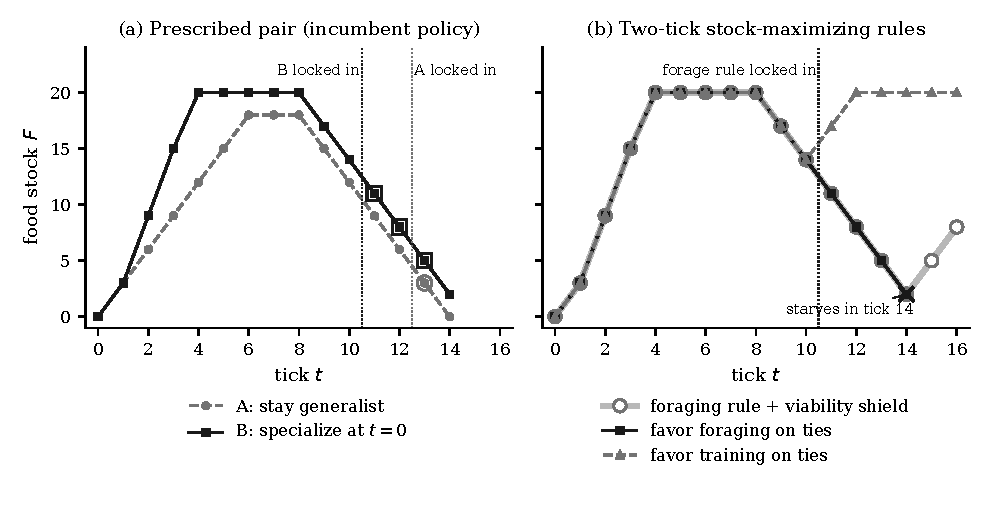
\includegraphics[width=\textwidth]{figures/fig_settlement.pdf}
\caption{The settlement paradox. (a)~Prescribed pair under the incumbent policy: generalist A and B, which specializes at $t=0$. Enlarged hollow markers show ticks at severity~3; dotted lines mark where each window has closed. (b)~Three rules maximizing food stored over the next two ticks; all specialize at tick~0. Favoring foraging on ties follows B into lock-in at tick~11 and starves in tick~14; favoring training reaches the horizon with 20 food; the shielded rule reaches it with 8. Recomputed with the repository's Python reference and checked against saved and certified values.}
\label{fig:settlement}
\end{figure}

\paragraph{Which rule selects B?} At each tick, score every admissible first action by its best continuation over the next two ticks (ticks survived, then summed ending stocks), execute it, and replan. Favoring \emph{foraging} on ties specializes at tick~0 and follows B into lock-in. Favoring \emph{training} on ties also specializes, but trains while storage is full (two workers at ticks 4 and 5, one at ticks 6 and 7), completes training during tick~8, holds 17 at tick~11, and reaches tick~16 with 20 food. A \emph{shielded} rule, the foraging rule restricted to actions whose next state stays in $\K_\adapt$, trains during ticks 10--12, when foraging produces nothing, acquires farming at tick~13 and finishes with 8 food; each override scores the same on the two-tick objective (Figure~\ref{fig:settlement}b). The rules diverge exactly when the specialist can redirect labor to training without losing food on its two-tick objective: when a full store would discard the surplus, or once wild yield has run out.

\subsection{Paradox pairs and a diagnostic fingerprint}

Two histories from a common $s_0$ form a \emph{paradox pair} for an objective $J$ if $J(h_B)\ge J(h_A)$ while $\mu(s^B_{t_1},t_1)<\mu(s^A_{t_1},t_1)$. This alone is the familiar efficiency--resilience tradeoff; the paradox proper is \emph{selection}, when a decision rule produces $h_B$. A pair is of \emph{resource type} if B's physical path dominates A's (so it works for every monotone $J$), \emph{strong} if at some tick B is at $\sigma=3$ while A is at $\sigma\le2$, and of \emph{externality type} if $J$ omits a viability-relevant burden. The settlement contains a selected, strong pair of resource type.

\begin{proposition}[Resources cannot by themselves worsen severity]\label{prop:resources}
Assume A0, A2 and organizational monotonicity (A4: from a richer $x$ with the same $(O,q)$, every admissible class-$k$ step is matched by one with a richer result and the same $(O,q)$). If $s=(x,O,\pi,q)$ and $s'=(x',O,\pi',q)$ with $x\succeq x'$, and switching between $\pi$ and $\pi'$ needs no implementation move, then $s'\in\K_k(t)\Rightarrow s\in\K_k(t)$ for $k\in\{\policy,\adapt,\phys\}$. Consequently, at any tick of a strong resource-type pair, $(O^B_t,q^B_t)\ne(O^A_t,q^A_t)$.
\end{proposition}

The fixed class is excluded because an incumbent's response to a richer state need not be monotone. The Lean statement requires equal $\pi$; the text relaxes this using immediate revision. Related comparison results for kernels under ordered dynamics are due to \citet{DeLaraEtAl2007} and \citet[Theorem~7]{DeLaraEtAl2020}. In the settlement the checks are exhaustive: across 1,362,312 same-$(O,q)$ pairs richer is never less recoverable, and all 22,484 strong-paradox state pairs differ in $(O,q)$.

\subsection{Prevalence and the price of safety}

\paragraph{Experiment E.} Over 6,000 settings (specialist retraining 1--10 worker-ticks with generalists at 2, specialization bonus 1--2, storage 12--30, horizon 12--20, 12 disturbance timings), the prescribed pair shows storage dominance with an earlier deadline in 1,581 settings (26.4\%), all with a strong severity gap; in 798 of them cumulative useful harvest ties, and no setting shows an earlier close without storage dominance. It never occurs when specialists clear training in one tick (0 of 1,800 settings), and occurs in 27.3\%, 41.7\% and 56.5\% of settings with 1, 2 and 3 extra ticks. Banking the surplus prevents it: prevalence is 61.3\% at capacity 12, 24.3\% at 20 and 0.4\% at 30, and 98.3\% with 3 extra ticks at capacity 12. The foraging-tie rule enters lock-in in 4,940 settings (82.3\%); the training-tie rule survives all 6,000. These frequencies describe the chosen grid, not real organizations.

\paragraph{Tie-breaking versus strict selection.} Because kernels are exact, a \emph{viability shield} in the sense of shielded reinforcement learning \citep{AlshiekhEtAl2018} is computable. Without friction, the shielded rule survives all 6,000 settings, overrides in exactly the 4,940 where the foraging rule locks in, and never lowers the two-tick objective; 10,750 of its 10,868 overrides occur after wild yield has run out, and 113 of the remaining 118 with storage full. Lock-in is thus a matter of tie-breaking. With a training cost of one food per trainee-tick, in every one of the 4,940 settings, at least one override lowers the two-tick objective, while the shield still survives all 6,000; the training-tie rule now survives only 2,075 settings, and a rule that acquires farming on ties and then specializes survives 660. In 523 settings the shield blocks specialization itself, because specializing at tick~0 leaves $\K_\adapt$ immediately while scoring strictly higher. At the forage rule's lock-in tick the shield holds on average 1.42 less food (stock plus incoming harvest), which understates the price: the deficit at that tick is zero in 1,316 settings because the shield's costs fall later: in 793 of them the trainee's food came from surplus a full store would have discarded, and in the other 523 the declined specialization bonus had not yet arrived. Skill decay (farming lost after $d$ consecutive ticks with no farmers) leaves the two-tick rules unchanged, since they farm every tick once farming is acquired, but with $d=2$ a rule that acquires farming as fast as possible and then specializes locks in 1,425 settings (3,160 with the training cost added). One food per trainee-tick is the model's smallest nonzero cost, so the threshold for strict selection cannot be located more finely. The paradox proper requires that acquiring the substitute capability cost something within the decision rule's lookahead.

\section{The necessity of acceleration}
\label{sec:accel}

\subsection{The delay theorem}

A component is \emph{irreversible} if no admissible action decreases it (cumulative CO$_2$ without removal). With lower burden ordered as better, Proposition~\ref{prop:resources} shows a heavier burden never helps in a cross-sectional comparison; the disadvantage can be offset by other components but never removed.

\begin{definition}[Rate classes and necessity]
For a ceiling $r$, $\U_r$ is the class of (possibly time-varying) capacity schedules whose growth never exceeds $r$, with kernel $\K_r(t)$; the classes are \emph{nested} if $r\le r'$ implies $\U_r\subseteq\U_{r'}$. The required rate is $r_{\mathrm{req}}(s,t)=\inf\{r:s\in\K_r(t)\}$. With incumbent rate $r_0$ and highest attainable rate $r_{\mathrm{cap}}$, acceleration is \emph{necessary} at $(s,t)$ if $s\in\K_{r_{\mathrm{cap}}}(t)\setminus\K_{r_0}(t)$.
\end{definition}

\begin{proposition}[Delay never lowers the required rate; Prop.~II.1 in the repository]\label{prop:delay}
If the rate classes are nested and the incumbent step is admissible at rate $r_0$, then for every $r\ge r_0$, $s\in\V$ and $t<T$: $b(s)\in\K_r(t+1)\Rightarrow s\in\K_r(t)$, where $b(s)$ is the state after one period of incumbent operation. Hence, along the incumbent trajectory before $t_\fail$, $\max(r_0,r_{\mathrm{req}})$ is nondecreasing.
\end{proposition}
\begin{proof}
The incumbent step lies in $\U_{r_0}\subseteq\U_r$; apply Proposition~\ref{prop:monotone} to $\U_r$.
\end{proof}

This is a direct consequence of the viability framework; the contribution is its application to deadlines for building capability. Stating necessity with kernels avoids the edge case where the infimum is not attained, and latency is already in the dynamics. The guards matter: the result concerns one fixed ceiling along the incumbent path under a known environment; it says nothing about ceilings below $r_0$, since a year of incumbent growth can make a lower rate suffice; and it does not say delaying \emph{any} intervention is harmful. Within these guards, waiting can turn a modest required acceleration into an unattainable one, never the reverse. Unlike rate-induced tipping \citep{WieczorekEtAl2011,AshwinEtAl2012}, the environment path is fixed and the varied rate is a ceiling on the system's responses. \emph{Nesting is substantive}: it fails when the environment reacts to the ceiling a system holds rather than the actions it takes (antitrust scrutiny triggered by capacity, a rival arming in response to capability). A higher ceiling can then shrink the kernel; Lean gives a three-state counterexample. In the climate model dynamics depend only on the rate used, so nesting holds.

The effective time of an intervention plan with shared resources is the makespan of a resource-constrained schedule, not its dependency-only critical path: two independent two-year tasks needing the same single manufacturing line take four years, and reorganizing informational dependencies cannot remove that physical bottleneck. Stages already represented in the dynamics are priced into the kernel, so the right tests are separate clocks: unmodeled stages (discovery, decision lag) must fit within the margin $\mu$; these plus building the capability must fit before $t^*_\phys$; and only all-or-nothing interventions need their full makespan, which a critical path \citep{KelleyWalker1959} only bounds from below, to fit before $t_\fail$. Interventions whose effect accumulates need not: at the climate model's NZE-consistent central settings the baseline exceeds the 2$^\circ$C budget in 2054, yet a viable 5\%/yr program started in 2027 deploys until net zero in 2062.

\subsection{A stylized climate application}

\paragraph{Model.} Annual steps 2027--2087. The physical state is the abated fraction $f$ of no-new-deployment emissions $E_{\mathrm{ref}}(t)=E_0\exp(\gamma\tau_d(1-e^{-t/\tau_d}))$ ($E_0=43.3$\,Gt, $\gamma=0.019$, $\tau_d=20$\,yr) and cumulative CO$_2$ $C$; organization is \emph{deployment capacity} $D$ (Gt/yr of abatement addable per year, $D_0=0.75$); commitments are capacity orders arriving after latency $L$. Net abatement cost is $n(f)=-50+490(e^{0.534f}-1)$ \$/t, and capex density is $c(f)=\psi(n(f)+100)\cdot25/1000$ with cost scale $\psi$. Spending is $Y_t=\varphi\cdot\$2.2\mathrm{T}\cdot1.025^t-c_{\mathrm{cap}}u_t$, so capacity orders $u_t$ (at $c_{\mathrm{cap}}=\$0.3$T per Gt/yr per yr) compete with deployment. Deployment advances $f$ as far as spending and capacity allow. A program with rate $r\le g_{\max}$ orders $rD_t$ while capacity binds; the incumbent uses 2\% at today's spending. Viability requires $C$ within the carbon budget every year and net zero by 2087.

\paragraph{Calibration status.} Emissions and remaining budgets from 2027 (510 and 1,035\,GtCO$_2$ for 1.7 and 2.0$^\circ$C at 50\%) are from the Global Carbon Budget 2026 \citep{FriedlingsteinEtAl2026}; robust budgets scale them by $0.45/0.63$, the worst case over the likely TCRE range \citep{IPCCWGISPM2021}; the \$2.2T anchor is the IEA estimate of 2026 clean-energy investment across many categories \citep{IEAWorldEnergyInvestment2026}; initial capacity is an assumption informed by \citet{EmberCapacity2026}. The cost curve is an assumed form fitted to two anchors informed by \citet{IPCCWGIIISPM2022}, the dollar-to-abatement conversion is assumed, and $\psi$ is swept, not estimated. ``NZE-consistent'' ($\psi=0.5$) means the model reaches net zero in 2050 after 444\,GtCO$_2$ at $\varphi=2$ with unlimited capacity.

\paragraph{Classes and exactness.} The policy class raises spending immediately (deliberately generous) but keeps the 2\% capacity rule; the adapt class allows any capacity schedule up to $g_{\max}$; a spending-bounded \emph{capacity-unconstrained} class substitutes for $\U_\phys$. Closing years are exact over all capacity schedules: constant-rate programs give witnesses, and a relaxed program with free capacity that grows at $g_{\max}$ unconditionally dominates every schedule, so by the Lean simulation theorem \lean{viab\_sim} its failure excludes them all (maximal deployment is dominant by \lean{greedy\_suffices}). The bounds agree in all 324 rate-window configurations, 576 comparison histories and 40 AI cells. The step-level dominance is proved on paper and checked numerically, not formalized.

\paragraph{Results.} The sweep covers 324 configurations over $\psi$, $\varphi$, $g_{\max}$, $L$, target and climate response; 1.5$^\circ$C is at $\sigma=4$ in every tested combination and excluded.
\begin{itemize}
\item \emph{Money alone is never enough}: in all 324 configurations, raising spending under the incumbent capacity rule fails.
\item \emph{The required rate rises with delay} (Figure~\ref{fig:climate}a). At the headline settings (central 2$^\circ$C, $\psi=0.5$, $\varphi=2$, $L=2$), 4\%/yr is excluded for all schedules from 2027 while 5\%/yr succeeds, so the incumbent's 2\% is insufficient; by 2040 the bracket is 23\%/24\%, and from 2043 no rate up to 100\% works. At $g_{\max}=30\%$ the last viable start is 2040; with unlimited capacity it is 2045, a five-year lock-in interval.
\item \emph{Across the sweep} (Figure~\ref{fig:climate}b), central 2$^\circ$C is open from 2027 in 72 of 81 configurations, with lock-in intervals of 2--8 years (median 4); robust 2$^\circ$C in 29 of 81, closing by 2034 at the latest, with 3--10 years (median 6). For 1.7$^\circ$C only one of 81 central settings (lowest costs, highest spending, 40\% scale-up, one-year lead time) admits a capacity-building path, from 2027 only. Dropping the net-zero condition changes none of the 18 headline closing years, and at the first excluded year the dominant program always fails by breaching the budget before 2087: the budget binds.
\item \emph{The binding constraint shifts.} Map four forms of acceleration onto the model: economic (spending $\varphi$), informational (cost scale $\psi$), material (maximum scale-up $g_{\max}$) and organizational (latency $L$). Over 108 one-step changes per axis, a step in $\psi$ or $\varphi$ moves the closing year by $+4.5$ years on average where the window is open before and after, a step in $g_{\max}$ by $+1.0$ and in $L$ by $+1.4$; no step closes an open window. Averages hide a regime change: at $\psi=1$ raising spending from 2 to 3 buys eight years (2029 to 2037), at $\psi=0.5$ only three (2040 to 2043), because at lower costs deployment capacity and the carbon budget bind. A ``step'' is a property of the grid, not of real-world difficulty; cost and spending enter almost only through their ratio, a limitation of the model; and without learning-by-doing the model may understate material acceleration.
\item \emph{AI as accelerator and margin consumer.} Incremental data-centre demand built from the IEA's projected rise from about 415\,TWh in 2024 to about 945\,TWh in 2030 \citep{IEAEnergyAI2025}, at an assumed 0.4\,tCO$_2$/MWh, shifts the closing year by zero or one year; high demand costs about a year and extreme demand about three, and a 10\% cost cut offsets high demand at both cost scales tested. Whether AI is net-positive for a window depends on which constraint it relieves and whether that constraint binds.
\item \emph{Externality-type tradeoff.} A prescribed carbon-price cutoff rule loses its 2$^\circ$C window in 58 of the 88 configurations where a capacity builder stays viable, while scoring at least as well as the builder at every annual prefix on a consumption proxy that omits damages. The price at which the cutoff path keeps its window is about \$100, \$200 and \$300/t at $\psi=0.5$, 0.75 and 1, close to the net cost of the last abatement tranche. The cutoff is prescribed, not optimized, so a selection claim would need a decision model.
\end{itemize}

\begin{figure}[t]
\centering
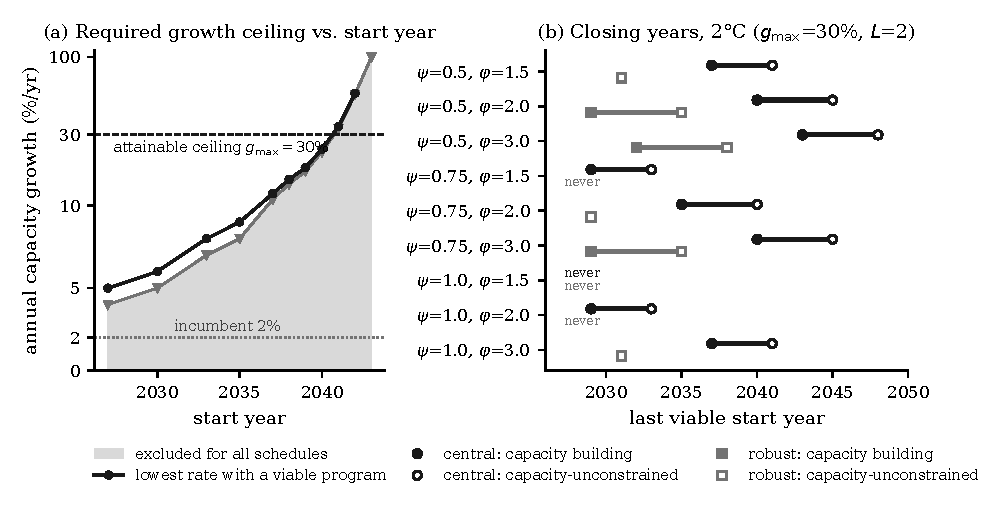
\includegraphics[width=\textwidth]{figures/fig_climate.pdf}
\caption{Climate recovery windows (stylized model; not a forecast). (a)~Headline settings: highest tested ceiling excluded for all schedules (shaded) and lowest constant rate with a viable program, by start year. (b)~Last viable start for capacity building (filled) and the capacity-unconstrained class (hollow), 2$^\circ$C, $g_{\max}=30\%$, $L=2$; the segment between them is the lock-in interval. Data: \texttt{results/argII\_output.txt}, \texttt{results/climate\_window.csv}.}
\label{fig:climate}
\end{figure}

\subsection{The acceleration dilemma}

Stopping capability growth is never viable for 2$^\circ$C in the model, and slowing it below the incumbent rate cannot help, since $\K_r\subseteq\K_{r_0}$ for $r<r_0$. Slowing \emph{pressure-generating} activity is different: it changes the environment path and lowers the required rate (removing extreme AI demand extends the window by three years). But faster capability building draws on the resources it is meant to enable, so the relevant object is the set of viable \emph{programs}. Programs that keep ordering capacity after it stops binding overbuild: they acquire an upper rate limit (13\%, 10\% and 8\% at $c_{\mathrm{cap}}=0.3,1,3$) and their windows close two to six years earlier than programs with a stopping rule, which remain viable up to the top of the tested range at moderate capacity costs (Figure~\ref{fig:corridor}). Proposition~\ref{prop:delay} concerns the full class under a ceiling; a prescribed grow-forever rule can even gain viability with delay (at $c_{\mathrm{cap}}=0.3$ it succeeds from 2027 at 5--13\%, and from 2038 at 15\%), because a later start leaves fewer years in which accumulated orders can exhaust spending.

Making speed itself costly, through a convex premium $c_{\mathrm{cap}}x_t(u_t/\bar g)^{\alpha-1}$ on orders implying growth $u_t$ above $\bar g=10\%$/yr, gives the stopping-rule program a real upper limit (at $c_{\mathrm{cap}}=1$, 44\% at $\alpha=2$ and 25\% at $\alpha=3$), but in every tested case it lies far above the lowest viable rate (5--6\%): a \emph{bounded corridor} whose closing year moves by at most two years. Embodied emissions of capacity spending penalize overbuilding, not speed: a stopping rule bounds total capacity by what can be used, so even 3\,GtCO$_2$ per \$T barely moves its window, whereas without a stopping rule they are decisive (at $c_{\mathrm{cap}}=1$ and 1\,GtCO$_2$ per \$T the grow-forever window closes in 2031 instead of 2036; at $c_{\mathrm{cap}}=3$ and the same intensity only 6\%/yr remains viable from 2027, and at 3\,GtCO$_2$ per \$T no tested rate does). These limits belong to prescribed programs, not to the class: under a ceiling a program may always order less, so raising the ceiling never shrinks the kernel. Selective acceleration therefore has two parts: which capabilities to accelerate (the binding ones) and when to stop.

\begin{figure}[t]
\centering
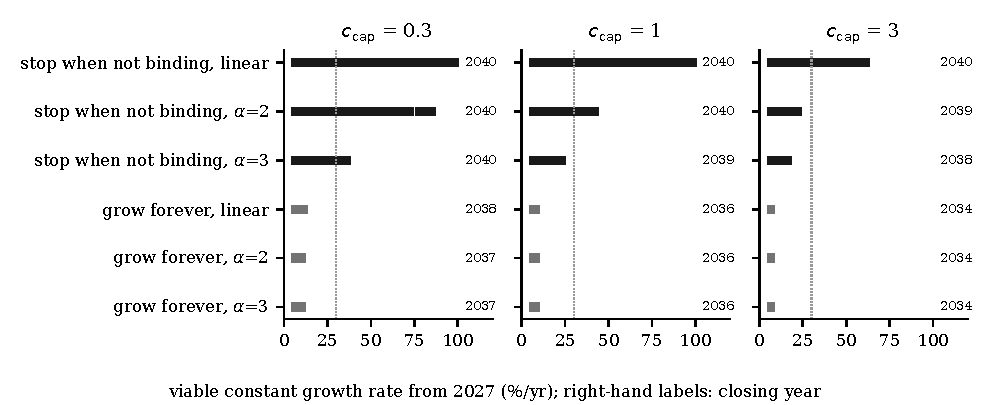
\includegraphics[width=\textwidth]{figures/fig_corridor.pdf}
\caption{The bounded corridor (central 2$^\circ$C, $\psi=0.5$, $\varphi=2$, $L=2$). Viable constant growth rates from 2027 for the program that stops ordering once capacity no longer binds (dark) and the program that grows forever (gray), under linear costs and convex ramp premiums with exponent $\alpha$, at three capacity costs. The gap at $c_{\mathrm{cap}}=0.3$, $\alpha=2$ is the failing 75\% rate (one order is unaffordable in 2032). Right-hand labels: closing year (rates up to $g_{\max}=30\%$, dotted). Recomputed with the Python reference and checked against \texttt{results/argII\_ramp\_output.txt}.}
\label{fig:corridor}
\end{figure}

\section{The adaptive escape problem}
\label{sec:escape}

\begin{definition}[Escape problem]
Given a class $\U$, sets $\W\subseteq\V$, horizon $T$ and state $s_0$, decide whether some $\U$-admissible continuation stays in $\V$ and ends in $\W$, and if so produce one.
\end{definition}

Escape is reach-avoid kernel membership with a witness. A finite-horizon escape is \emph{sustainably} successful if its terminal state also lies in the infinite-horizon kernel; the condition is placed on the terminal state rather than on $\W$ because under A0 an $x$-only terminal set contains states whose organization cannot keep $x$ there. For environments that keep changing, finite-horizon escape renewed as the horizon advances is the right target. Membership in $\K_\adapt$ entails physical feasibility (Proposition~\ref{prop:nesting}) and \emph{adaptive continuity}: the system must stay viable while it reorganizes, with transitional restrictions charged on the tick each move is made. The locked-in specialists of Table~\ref{tab:states} fail exactly this requirement.

\subsection{Hardness and tractable structure}

\begin{theorem}[Planning reduces to escape]\label{thm:escape}
Given a propositional STRIPS instance with positive preconditions and a positive conjunctive goal, make propositions capabilities and operators moves (plus the null move); add a physical bit $x$, initially 0, with $\W_x=\{1\}$ and $\V$ the whole space; and add an action \emph{declare}, admissible only when all goal capabilities are present, that sets $x=1$ irreversibly. Then a plan of length at most $n$ exists if and only if the organization can escape in exactly $n+1$ steps.
\end{theorem}
\begin{proof}[Proof sketch]
Machine-checked (\lean{Escape.planning\_iff\_escape\_A0}). Follow the plan, declare, then wait; conversely, the non-null moves before declaration form a plan.
\end{proof}

\begin{corollary}\label{cor:pspace}
\citet[Theorem~4.1]{Bylander1994} proves bounded STRIPS plan existence PSPACE-complete, already with two positive preconditions and two postconditions per operator; the hardness proof uses bounds of size $2^n$, so the bound must be written in binary. Because the mapping adds one move, one bit and one action, deciding escape with a binary-encoded horizon is PSPACE-hard.
\end{corollary}

Negative goal literals can be compiled into fresh complement propositions without changing plan lengths. The equivalence is machine-checked; the polynomial encoding is argued, not formalized. \citet{AbdulazizKurz2023} earlier machine-checked a bounded planning encoding in Isabelle/HOL. The hardness comes from compositional description ($n$ capabilities, $2^n$ organizations); with explicitly listed states, as in the settlement, escape is graph search.

For deterministic finite instances with a unary or polynomially bounded horizon and polynomial-time checkable dynamics, a guessed continuation is verifiable in polynomial time; with a variable unary horizon the problem is NP-complete for a class containing these instances. The lower bounds concern worst-case families, not the difficulty of a particular organizational model. Three structures support exact computation here: explicit state spaces (backward recursion, linear in time-indexed states times actions), monotone dynamics with a dominant rule (one simulation per query; the climate certificate), and monotone capability acquisition.

\begin{theorem}[Monotone acquisition is tractable]\label{thm:horn}
If every move only adds capabilities and requires only that certain capabilities be present, with no binding step limit, no resource competition and no risk of leaving $\V$, then a state containing all requested capabilities is reachable if and only if each lies in the closure of the seeds under the moves, and forward chaining computes that closure in time linear in the total size of the explicit rules and seeds.
\end{theorem}

Each prerequisite alternative is a definite Horn rule, and the counter-and-queue algorithm of \citet{DowlingGallier1984} gives the linear bound. A deadline breaks this: one move per tick over Set Cover moves makes the bounded problem NP-complete even without deletions or prerequisites \citep{Karp1972}, though the unbounded closure still certifies exclusion of every capability outside it. Polytree causal graphs of bounded indegree are another tractable case \citep{BrafmanDomshlak2003}; without the indegree bound binary polytrees are NP-complete \citep[Theorem~6.3]{GimenezJonsson2008}.

\subsection{Restoration independence}

Recovery may depend on capabilities disabled by the same disruption, as when restarting a grid requires generating without external power. Each capability has alternative prerequisite sets and can be restored once every member of one alternative is up; a set $R$ is \emph{independently recoverable} from survivors $S$ if $R\subseteq\mathrm{closure}(S)$, decidable in linear time by Theorem~\ref{thm:horn} when restoration has no deadline or resource competition. \emph{Redundancy is not independence}: in a stylized six-capability grid in which generators need control and fuel, control needs power and telecom, telecom and fuel need power, and power needs a generator, a total blackout restores 0 of 6 capabilities, adding a third generator restores 0 of 7, and a single black-start hydro unit restores 7 of 7, because only it breaks the dependency cycle.

\begin{theorem}[Restoration seeds under conjunctive prerequisites]\label{thm:fvs}
If each capability has a single prerequisite set, then $\mathrm{closure}(S)$ contains every capability if and only if $S$ meets every directed cycle of the dependency graph; finding a minimum such $S$ is the minimum directed feedback vertex set problem, which is NP-hard \citep{Karp1972}.
\end{theorem}

This is the unanimous-threshold case of the directed target-set characterization of \citet{FeigeKogan2021} (Theorem~3.10 in the arXiv preprint version), restated in restoration terms. Checking a seed set is linear-time; choosing a smallest one is hard.

\paragraph{Closure is a screen, not a schedule.} For a chain $B\to P\to G\to E$ with seed $\{B\}$, $E$ is in the closure. Let activation be serial ($\tau(P)=3$, $\tau(G)=4$, $\tau(E)=3$ powered ticks), and let power come from $B$ only for ticks $t<L$, or from $E$ once online. For every $L\le9$, $E$ is unreachable at every horizon; for $L\in\{10,11,12\}$ it is online at tick 10. Lean proves both (\lean{timed\_unreachable\_of\_short\_seed}, \lean{timed\_bootstrap\_reachable\_long\_seed}). Static closure is therefore a necessary screen: outside it no schedule restores a capability; inside it, feasibility depends on durations, capacities and how long the seed lasts, which is the timed machinery of Sections~\ref{sec:framework} and~\ref{sec:accel}. The prerequisite graph must also be visible to the controller; otherwise a stabilizing action, such as shedding a load a prerequisite depends on, can disable it unnoticed, an instance of informational rather than organizational lock-in.

\begin{lemma}[Seed undervaluation]\label{lem:seed}
If a robust optimizer scores actions by their worst case over a finite disturbance set, and on every disturbance in the set a seed pays the alternative's payoff minus a cost $c$, then the seed's relative robust value is exactly $-c$; with $c>0$ it is never selected.
\end{lemma}

This is machine-checked (\lean{robust\_seed\_value}, \lean{robust\_never\_picks\_seed}); \lean{seed\_example} shows the optimizer buying the seed once a cycle-breaking disturbance is added. An organization optimized against a modeled threat set is stripped of the capability that would protect it against the rest, one formal route to ``robust yet fragile'' \citep{CarlsonDoyle2002}. Restoration independence must be imposed as a structural requirement.

\subsection{Bounds and the gap}

Following the distinction between plans and unsolvability certificates \citep[Definitions~1--2]{ErikssonEtAl2017}, witnesses prove kernel membership, certificates prove exclusion, and the \emph{gap} is what has neither. Since any relaxation containing $\K_\phys$ accepts every lock-in state, certifying lock-in needs evidence that distinguishes organizationally admissible trajectories. We classify all 17,136 settlement states using budget-limited random search for adapt-class witnesses under two certificates: the exact physical class, and an organizational relaxation in which training does not take workers off production (Table~\ref{tab:gap}).

\begin{table}[t]
\centering\small
\caption{Witness/certificate bracketing over the settlement state space, scored against the exact kernels.}
\label{tab:gap}
\begin{tabular}{@{}lrrrrrr@{}}
\toprule
Certificate & Rollouts/state & Witness & Excluded & Unknown & Unknown, $\sigma=3$ & Wrong \\
\midrule
physical & 1 & 9,906 & 384 & 6,846 & 1,178 & 0 \\
physical & 1,000 & 15,373 & 384 & 1,379 & 1,178 & 0 \\
relaxation & 1 & 9,901 & 1,470 & 5,765 & 92 & 0 \\
relaxation & 1,000 & 15,374 & 1,470 & 292 & 92 & 0 \\
\bottomrule
\end{tabular}
\end{table}

The physical certificate leaves all 1,178 lock-in states unresolved at every budget; at 1,000 rollouts, 1,379 states are unresolved, including 201 recoverable ones. The relaxation alone excludes 1,470 states from $\K_\adapt$, establishing only $\sigma\in\{3,4\}$; paired with the exact physical kernel, 1,086 of them (92\% of the lock-in states) have a physical witness and are certified lock-in, and the other 384 are the $\sigma=4$ states. About 200 recoverable states still lack a witness at 1,000 rollouts, which a better search could reduce. No claim in any run was wrong: the bracketing is honest about what it does not know.

\paragraph{An anytime escape strategy.} Given the hardness results, escape is best pursued by an anytime bounding loop: observe, bound the question with witnesses and certificates, locate deadlines and the required rate, diagnose the cause from the severity interval (policy at $\sigma=1$, missing capability at 2, inaccessible alternatives at 3, physics at 4), act on the best witness, prefer interventions that preserve margin and recoverable closure, and update. Severities 3 and 4, and ``unknown,'' are legitimate outputs. Where kernels are exact, preserving options takes the form of the viability shield of Section~\ref{sec:paradox}; where they are only bounded, a shield must use an inner approximation and the gap becomes the cost of caution.

\section{Related work}
\label{sec:related}

\paragraph{Lock-in and recoverability.} The kernel construction rests on target tubes \citep{BertsekasRhodes1971} and viability theory \citep{Aubin1991}. \citet{HeitzigEtAl2016} classify states by what default dynamics and management can sustain, and \citet{KittelEtAl2021} compute that topology with viability algorithms. Closest is \citet{PichancourtEtAl2025}, who compute finite-horizon viability along governance pathways distinguishing operational, collective-choice and constitutional changes; their levels concern who may change rules, whereas our classes ask which kind of intervention suffices at a fixed state and deadline. \citet{SoentgesEtAl2018} compute the last admissible maneuver along a vehicle trajectory, \citet{Lofberg2012} studies recursive feasibility of a given receding-horizon law, and adaptation tipping points in dynamic adaptive policy pathways \citep{HaasnootEtAl2013} mark when an action stops meeting objectives; our class-specific deadline is instead the last baseline state from which some continuation in an entire class can meet the criterion. Organizationally, core rigidities \citep{LeonardBarton1992}, exploitation crowding out exploration \citep{March1991} and capability traps \citep{RepenningSterman2002} describe the phenomenon, and \citet{HannanEtAl2003} relate architecture to reorganization time and mortality, a possible origin for the retraining costs the settlement takes as inputs.

\paragraph{Deadlines and rates.} \citet[Section~4 and Figure~4]{PetschelHeldEtAl1999} relate waiting time, transition time and sustained reduction rates under guardrails; \citet{Stocker2013} shows how delay raises the required mitigation rate; \citet{vanZalingeEtAl2017} and \citet[Sections~2--3]{AengenheysterEtAl2018} compute climate points of no return; \citet{IyerEtAl2015} vary action timing and technology diffusion limits; and \citet{VogtSchilbHallegatte2014} show how deployment speed affects optimal mitigation timing. \citet{MathiasEtAl2017} trace the loss of feasible policies as departure from business as usual is delayed. \citet{BottaEtAl2017} formalize finite-horizon reachability, viability and avoidability for sequential decisions, with climate applications to uncertain emission policies \citep{BottaEtAl2018}; there viability means a process can continue for a number of steps, whereas we require stated safety and terminal conditions. \citet{StrnadEtAl2019} search governance sequences with reinforcement learning; in their Figure~5 the agent subsidizes renewables for most of the run, and a carbon tax cannot be introduced immediately without breaching the social-foundation boundary and is switched on only later. Their action menu is fixed in advance; we ask when changing the organization can still make a different action available before the deadline. Our other additions are the nesting condition under which the delay result transfers across models, and capacity orders that compete with deployment and deliver after a lag. On terminology, carbon lock-in \citep{Unruh2000} concerns technologies and institutions sustained by increasing returns; our use of \emph{lock-in} always specifies the horizon, target and relaxed interventions.

\paragraph{Planning, restoration and certificates.} The hardness transfer rests on \citet{Bylander1994}, the restoration characterization on \citet{FeigeKogan2021}, closure on \citet{DowlingGallier1984}, unsolvability certificates on \citet{ErikssonEtAl2017}, and shields on \citet{AlshiekhEtAl2018}. Machine-checked planning encodings precede ours \citep{AbdulazizKurz2023}.

\section{Limitations}
\label{sec:limits}

\paragraph{Existence, not prevalence.} The settlement fixes retraining costs of 8 versus 2. The tradeoff recurs in 26.4\% of the chosen grid, but whether real organizations acquire such latencies or use comparable decision rules is empirical.

\paragraph{Selection is tie-breaking without friction.} A shield saves every frictionless setting at no cost on the two-tick objective; strict selection needs a training cost.

\paragraph{The physical class is idealized} by design, so the gap to $\K_\adapt$ measures the cost of having to learn. A less idealized physical class can be substituted under A3 or A3$'$.

\paragraph{The climate model is stylized}: one sector and capability, a smooth cost curve, linear TCRE, no damages, tipping, regions or political economy. Its incumbent is optimistic (roughly 2.1--2.4$^\circ$C by 2100, below published current-policy projections of about 2.6--2.8$^\circ$C), and asset replacement is free, so results lean toward understating difficulty. Results depend most on $\psi$ and $\varphi$, the least identified parameters. Necessity is conditional even within the model: in 9 of the 81 central 2$^\circ$C configurations no attainable rate works from 2027.

\paragraph{Formal scope.} \lean{native\_decide} trusts the compiler; theory and certified model are not linked; the climate implementation is not proved to instantiate the abstract system, and its terminal condition is not formalized; the complexity encoding is argued, not formalized.

\section{Conclusion}
\label{sec:conclusion}

An adaptive system cannot be evaluated by its current productive capability alone; its organization determines which future states remain reachable, and for how long. In an exact model, a stock-maximizing rule exhausts its recovery window while still holding more food than a generalist that can recover. Necessity of acceleration is a kernel condition, waiting under an unchanged ceiling can only raise the required rate, and how a system accelerates matters as much as how fast. Escape inherits planning hardness, yet structure permits exact or bracketed computation, and lock-in requires both a physical witness and an organizational exclusion: diagnosis, time constraint, and intervention.

\bibliographystyle{plainnat}
\bibliography{references}

\appendix

\section{Machine-checked results}
\label{app:lean}

Table~\ref{tab:lean} lists the Lean~4 files (Lean 4.15.0, no dependencies; library files in \texttt{Paradox/}) and principal theorem names, with trust levels as stated in the repository README.

\begin{table}[ht]
\centering\footnotesize
\caption{Lean files, theorem names and trust levels.}
\label{tab:lean}
\begin{tabular}{@{}L{1.1in}L{3.05in}L{1.95in}@{}}
\toprule
File & Theorems (paper result) & Trust level \\
\midrule
\lean{Theory.lean} &
\lean{viab\_sim}; \lean{nesting}, \lean{nesting\_dominance} (Prop.~\ref{prop:nesting}); \lean{monotone\_loss}, \lean{loss\_permanent} (Prop.~\ref{prop:monotone}); \lean{robust\_strengthened}, \lean{robust\_monotone\_loss\_fails} (robust analogue and counterexample); \lean{resources\_monotone}, \lean{paradox\_fingerprint} (Prop.~\ref{prop:resources}); \lean{greedy\_suffices}; \lean{rate\_upward}, \lean{delay\_never\_lowers\_required\_rate} (Prop.~\ref{prop:delay}); \lean{cap\_not\_nested}, \lean{cap\_kernel\_shrinks}, \lean{rate\_upward\_needs\_nesting}; \lean{robust\_seed\_value}, \lean{robust\_never\_picks\_seed}, \lean{seed\_example} (Lemma~\ref{lem:seed}) &
Fully proved; no \lean{sorry}, no \lean{native\_decide}. Axioms: none, or only \lean{propext} and \lean{Quot.sound} (from \lean{omega}) \\
\addlinespace
\lean{Escape.lean} &
\lean{escape\_wait}; \lean{planning\_iff\_escape}; \lean{planning\_iff\_escape\_A0} (Theorem~\ref{thm:escape}) &
Fully proved; no \lean{sorry}, no \lean{native\_decide}. Axioms: \lean{propext}, \lean{Quot.sound} only \\
\addlinespace
\lean{Timed.lean} &
\lean{timed\_bootstrap\_static\_reachable}; \lean{timed\_unreachable\_of\_short\_seed}; \lean{timed\_bootstrap\_timed\_unreachable}; \lean{timed\_bootstrap\_reachable\_long\_seed} &
Fully proved; no \lean{sorry}, no \lean{native\_decide}. Axioms: \lean{propext}, \lean{Classical.choice}, \lean{Quot.sound} \\
\addlinespace
\lean{Model.lean} &
\lean{Params.step\_valid}: every successful step preserves the state invariant, for all training thresholds, decay settings and training costs &
Proved in general \\
\addlinespace
\lean{Certified.lean} &
\lean{sigma0}--\lean{sigma4}; \lean{witnesses\_verify}; \lean{state\_count}; \lean{no\_nesting\_violations}; \lean{B\_dominates\_storage}; \lean{windows}; \lean{strong\_at\_11}; \lean{stock\_decisions}; \lean{prop4\_check}; \lean{fingerprint\_check} &
Certified for one model by \lean{native\_decide}, which trusts the Lean compiler (\lean{Lean.ofReduceBool}) \\
\addlinespace
\lean{Kernel}, \lean{Decision}, \lean{Friction}, \lean{Climate}; executables &
Exact kernels, decision rules, Experiment E, friction sweep, climate sweeps, Argument II and III experiments &
Numerical; outputs reproduced by the independent Python reference \\
\bottomrule
\end{tabular}
\end{table}

\section{Reproducibility}
\label{app:repro}

The artifact (\url{https://github.com/Patrick-Barletta/Paradox_of_Adaptive_Organization}, tag v1.0) needs Lean 4.15.0 and Python~3 with the standard library. \texttt{lake build} compiles all proofs, certified facts and executables; on Windows, \texttt{.\textbackslash run\_all.ps1} builds everything and regenerates the saved outputs in \texttt{results/}. \texttt{python python/crosscheck\_all.py} recomputes every result with the independent Python reference and compares it with the saved files (324 climate-window and 288 climate-comparison rows, eight text reports line by line, and all 6,000 Experiment E settings), exiting nonzero on any mismatch. The run log records clean rebuilds with identical SHA-256 hashes and byte-identical regeneration of every previously saved output after each extension. The figures here are produced by \texttt{preprint/figures/make\_figures.py}, which asserts agreement with the saved numbers before plotting.

\end{document}
